\documentclass[mathserif]{beamer}

\setbeamertemplate{frametitle}[default][center]%Centers the frame title.
\setbeamertemplate{navigation symbols}{}%Removes navigation symbols.
\setbeamertemplate{footline}{\raisebox{5pt}{\makebox[\paperwidth]{\hfill\makebox[10pt]{\scriptsize\insertframenumber}}}}
\setbeamertemplate{caption}[numbered]

%\newcommand{\tth}   {\mbox{$\theta$}}
\newcommand{\thh}   {\mbox{$\theta$}}
\newcommand{\su}   {\mbox{$\sigma^2$}}
\newcommand{\so}   {\mbox{$\sigma_0^2$}}
\newcommand{\ko}   {\mbox{$\kappa_0$}}
\newcommand{\no}   {\mbox{$\nu_0$}}
\newcommand{\mo}   {\mbox{$\mu_0$}}
\newcommand{\ti}   {\mbox{$\tilde{x}$}}
\newcommand{\la}   {\mbox{$\lambda$}}
\newcommand{\bx}   {\mbox{$\bm{x}$}}
\newcommand{\bZ}   {\mbox{$\bm{Z}$}}
\newcommand{\bX}   {\mbox{$\bm{X}$}}
\newcommand{\bY}   {\mbox{$\bm{Y}$}}
\newcommand{\bA}   {\mbox{$\bm{A}$}}
\newcommand{\ba}   {\mbox{$\bm{a}$}}
\newcommand{\bb}   {\mbox{$\bm{b}$}}
\newcommand{\bt}   {\mbox{$\bm{t}$}}
\newcommand{\bz}   {\mbox{$\bm{z}$}}
\newcommand{\bw}   {\mbox{$\bm{w}$}}
\newcommand{\bbeta}   {\mbox{$\bm{\beta}$}}

\newcommand{\be}   {\mbox{$\bm{e}$}}
\newcommand{\bu}   {\mbox{$\bm{u}$}}
\newcommand{\bv}   {\mbox{$\bm{v}$}}
\newcommand{\sig}   {\mbox{$\Sigma$}}
\newcommand{\sigx}   {\mbox{$\Sigma_{XX}$}}
\newcommand{\sigxy}   {\mbox{$\Sigma_{XY}$}}
\newcommand{\tr}   {\mbox{$\text{tr}$}}
\newcommand{\ddet}   {\mbox{$\text{det}$}}
\newcommand\independent{\protect\mathpalette{\protect\independenT}{\perp}}
\def\independenT#1#2{\mathrel{\rlap{$#1#2$}\mkern2mu{#1#2}}}

\newcommand{\Expect}[1]{\ensuremath{\mathbf{E}\left[ #1 \right]}}
%\newcommand{\Var}[1]{\ensuremath{\mathrm{Var}\left[ #1 \right]}}
%\newcommand{\Cov}[1]{\ensuremath{\mathrm{Cov}\left[ #1 \right]}}
\newcommand{\MSE}{\ensuremath{\mathrm{MSE}}}
\newcommand{\RSS}{\ensuremath{\mathrm{RSS}}}
\newcommand{\Prob}[1]{\ensuremath{\mathrm{Pr}\left( #1 \right)}}
\newcommand{\ProbEst}[1]{\ensuremath{\widehat{\mathrm{Pr}}\left( #1 \right)}}
\DeclareMathOperator*{\argmin}{argmin} % thanks, wikipedia!
\DeclareMathOperator*{\argmax}{argmax} % thanks, wikipedia!
\DeclareMathOperator*{\sgn}{sgn} % thanks, wikipedia!

\newcommand{\lam}{\lambda}
\newcommand{\bmu}{\bm{\mu}}
%\newcommand{\bx}{\ensuremath{\mathbf{X}}}
\newcommand{\X}{\ensuremath{\mathbf{X}}}
\newcommand{\w}{\ensuremath{\mathbf{w}}}
\newcommand{\h}{\ensuremath{\mathbf{h}}}
\newcommand{\V}{\ensuremath{\mathbf{V}}}
%\newcommand{\tr}{\operatorname{tr}}

%\newcommand{\bx}{\ensuremath{\mathbf{X}}}
%\newcommand{\X}{\ensuremath{\mathbf{x}}}
%\newcommand{\w}{\ensuremath{\mathbf{w}}}
%\newcommand{\h}{\ensuremath{\mathbf{h}}}
%\newcommand{\V}{\ensuremath{\mathbf{v}}}
%\newcommand{\Cov}{\text{Cov}}
%\newcommand{\Var}{\text{Var}}

\DeclareMathOperator{\var}{Var}
\DeclareMathOperator{\cov}{Cov}
\newcommand{\Var}[1]{\ensuremath{\mathrm{Var}\left[ #1 \right]}}
\newcommand{\Cov}[1]{\ensuremath{\mathrm{Cov}\left[ #1 \right]}}


\newcommand{\indep}{\rotatebox{90}{\ensuremath{\models}}}
\newcommand{\notindep}{\not\hspace{-.05in}\indep}







\usepackage{float,bm}
\floatstyle{boxed}
\newfloat{code}{tp}{code}
\floatname{code}{Code Example}
\newcommand{\tth}   {\mbox{$\theta$}}
\newcommand{\thh}   {\mbox{$\theta$}}
\newcommand{\su}   {\mbox{$\sigma^2$}}
\newcommand{\so}   {\mbox{$\sigma_0^2$}}
\newcommand{\ko}   {\mbox{$\kappa_0$}}
\newcommand{\no}   {\mbox{$\nu_0$}}
\newcommand{\mo}   {\mbox{$\mu_0$}}
\newcommand{\ti}   {\mbox{$\tilde{x}$}}
\newcommand{\la}   {\mbox{$\lambda$}}
\newcommand{\bx}   {\mbox{$\bm{x}$}}
\newcommand{\bZ}   {\mbox{$\bm{Z}$}}
\newcommand{\bX}   {\mbox{$\bm{X}$}}
\newcommand{\bY}   {\mbox{$\bm{Y}$}}
\newcommand{\bA}   {\mbox{$\bm{A}$}}
\newcommand{\ba}   {\mbox{$\bm{a}$}}
\newcommand{\bb}   {\mbox{$\bm{b}$}}
\newcommand{\bt}   {\mbox{$\bm{t}$}}
\newcommand{\bz}   {\mbox{$\bm{z}$}}
\newcommand{\bw}   {\mbox{$\bm{w}$}}
\newcommand{\bbeta}   {\mbox{$\bm{\beta}$}}

\newcommand{\be}   {\mbox{$\bm{e}$}}
\newcommand{\bu}   {\mbox{$\bm{u}$}}
\newcommand{\bv}   {\mbox{$\bm{v}$}}
\newcommand{\sig}   {\mbox{$\Sigma$}}
\newcommand{\sigx}   {\mbox{$\Sigma_{XX}$}}
\newcommand{\sigxy}   {\mbox{$\Sigma_{XY}$}}
\newcommand{\tr}   {\mbox{$\text{tr}$}}
\newcommand{\ddet}   {\mbox{$\text{det}$}}
\newcommand\independent{\protect\mathpalette{\protect\independenT}{\perp}}
\def\independenT#1#2{\mathrel{\rlap{$#1#2$}\mkern2mu{#1#2}}}

\newcommand{\Expect}[1]{\ensuremath{\mathbf{E}\left[ #1 \right]}}
%\newcommand{\Var}[1]{\ensuremath{\mathrm{Var}\left[ #1 \right]}}
%\newcommand{\Cov}[1]{\ensuremath{\mathrm{Cov}\left[ #1 \right]}}
\newcommand{\MSE}{\ensuremath{\mathrm{MSE}}}
\newcommand{\RSS}{\ensuremath{\mathrm{RSS}}}
\newcommand{\Prob}[1]{\ensuremath{\mathrm{Pr}\left( #1 \right)}}
\newcommand{\ProbEst}[1]{\ensuremath{\widehat{\mathrm{Pr}}\left( #1 \right)}}
\DeclareMathOperator*{\argmin}{argmin} % thanks, wikipedia!
\DeclareMathOperator*{\argmax}{argmax} % thanks, wikipedia!
\DeclareMathOperator*{\sgn}{sgn} % thanks, wikipedia!

\newcommand{\lam}{\lambda}
\newcommand{\bmu}{\bm{\mu}}
%\newcommand{\bx}{\ensuremath{\mathbf{X}}}
\newcommand{\X}{\ensuremath{\mathbf{X}}}
\newcommand{\w}{\ensuremath{\mathbf{w}}}
\newcommand{\h}{\ensuremath{\mathbf{h}}}
\newcommand{\V}{\ensuremath{\mathbf{V}}}
%\newcommand{\tr}{\operatorname{tr}}

%\newcommand{\bx}{\ensuremath{\mathbf{X}}}
%\newcommand{\X}{\ensuremath{\mathbf{x}}}
%\newcommand{\w}{\ensuremath{\mathbf{w}}}
%\newcommand{\h}{\ensuremath{\mathbf{h}}}
%\newcommand{\V}{\ensuremath{\mathbf{v}}}
%\newcommand{\Cov}{\text{Cov}}
%\newcommand{\Var}{\text{Var}}

\DeclareMathOperator{\var}{Var}
\DeclareMathOperator{\cov}{Cov}
\newcommand{\Var}[1]{\ensuremath{\mathrm{Var}\left[ #1 \right]}}
\newcommand{\Cov}[1]{\ensuremath{\mathrm{Cov}\left[ #1 \right]}}


\newcommand{\indep}{\rotatebox{90}{\ensuremath{\models}}}
\newcommand{\notindep}{\not\hspace{-.05in}\indep}






%\usepackage{fontspec}
%\setmainfont{Tahoma}

\newcommand{\del}   {\mbox{$\delta(x)$}}

%\newcommand{\lam}{\lambda}
%\newcommand{\bmu}{\bm{\mu}}
%%\newcommand{\bx}{\ensuremath{\mathbf{X}}}
%\newcommand{\X}{\ensuremath{\mathbf{x}}}
%\newcommand{\w}{\ensuremath{\mathbf{w}}}
%\newcommand{\h}{\ensuremath{\mathbf{h}}}
%\newcommand{\V}{\ensuremath{\mathbf{v}}}
%\newcommand{\cov}{\text{Cov}}
%\newcommand{\var{\text{Var}}}

%\DeclareMathOperator{\var}{Var}
%\DeclareMathOperator{\cov}{Cov}

%\newcommand{\indep}{\rotatebox{90}{\ensuremath{\models}}}
%\newcommand{\notindep}{\not\hspace{-.05in}\indep}

%\newcommand{\bX}   {\mbox{$\bm{X}$}}
%\newcommand{\bx}   {\mbox{$\bm{x}$}}
%\newcommand{\V}   {\mbox{\text{Var}}}
%\newcommand{\tth}   {\mbox{$\theta$}}
%\newcommand{\su}   {\mbox{$\sigma^2$}}
%\newcommand{\so}   {\mbox{$\sigma_0^2$}}
%\newcommand{\ko}   {\mbox{$\kappa_0$}}
%\newcommand{\no}   {\mbox{$\nu_0$}}
%\newcommand{\mo}   {\mbox{$\mu_0$}}
%\newcommand{\ti}   {\mbox{$\tilde{x}$}}
%\newcommand{\la}   {\mbox{$\lambda$}}

\newtheoremstyle{example}
{\topsep} % space above
{\topsep} % space below
{} % body font
{} % indent
{\bf} % head font
{:} % punctuation between head and body
{0.5em} % space after head
{} % manually specify head
%{\thmname{#1}\thmnumber{ #2}\thmnote{:#3}} % manually specify head



\newtheoremstyle{definition}
{\topsep} % space above
{\topsep} % space below
{} % body font
{} % indent
{\bf} % head font
{:} % punctuation between head and body
{0.5em} % space after head
{} % manually specify head
%{\thmname{#1}\thmnumber{ #2}\thmnote{:#3}} % manually specify head

\newtheoremstyle{algorithm}
{\topsep} % space above
{\topsep} % space below
{} % body font
{} % indent
{\bf} % head font
{:} % punctuation between head and body
{0.5em} % space after head
{} % manually specify head
%{\thmname{#1}\thmnumber{ #2}\thmnote{:#3}} % manually specify head



\newtheoremstyle{theorem}
{\topsep} % space above
{\topsep} % space below
{} % body font
{} % indent
{\bf} % head font
{:} % punctuation between head and body
{0.5em} % space after head
{} % manually specify head
%{\thmname{#1}\thmnumber{ #2}\thmnote{:#3}} % manually specify head




\usepackage{graphicx} %The mode "LaTeX => PDF" allows the following formats: .jpg  .png  .pdf  .mps
\graphicspath{{./PresentationPictures/}} %Where the figures folder is located
\usepackage{listings}
\usepackage{media9}
\usepackage{movie15}
\addmediapath{./Movies/}

\newcommand{\beginbackup}{
   \newcounter{framenumbervorappendix}
   \setcounter{framenumbervorappendix}{\value{framenumber}}
}
\newcommand{\backupend}{
   \addtocounter{framenumbervorappendix}{-\value{framenumber}}
   \addtocounter{framenumber}{\value{framenumbervorappendix}} 
}


%\usepackage{algorithm2e}
\usepackage[ruled,lined]{algorithm2e}
\def\algorithmautorefname{Algorithm}
\SetKwIF{If}{ElseIf}{Else}{if}{then}{else if}{else}{endif}
%\usepackage{times}
%\usepackage[tbtags]{amsmath}
%\usepackage{amssymb}
\usepackage{amsfonts}
%\usepackage{slfortheorems}
\usepackage{epsfig}
\usepackage{graphicx}
\usepackage[small]{caption}
%\usepackage[square]{natbib}
%\newcommand{\newblock}{}
%\bibpunct{(}{)}{;}{a}{}{,}
%\bibliographystyle{ims}
%\usepackage[letterpaper]{geometry}
\usepackage{color}
\setlength{\parindent}{0pt}

\usepackage{natbib}
\bibpunct{(}{)}{;}{a}{}{,}
%\usepackage{hyperref}



%\usepackage{zref-savepos}
%
%\newcounter{restofframe}
%\newsavebox{\restofframebox}
%\newlength{\mylowermargin}
%\setlength{\mylowermargin}{2pt}
%
%\newenvironment{restofframe}{%
%    \par%\centering
%    \stepcounter{restofframe}%
%    \zsavepos{restofframe-\arabic{restofframe}-begin}%
%    \begin{lrbox}{\restofframebox}%
%}{%
%    \end{lrbox}%
%    \setkeys{Gin}{keepaspectratio}%
%    \raisebox{\dimexpr-\height+\ht\strutbox\relax}[0pt][0pt]{%
%    \resizebox*{!}{\dimexpr\zposy{restofframe-\arabic{restofframe}-begin}sp-\zposy{restofframe-\arabic{restofframe}-end}sp-\mylowermargin\relax}%
%        {\usebox{\restofframebox}}%
%    }%
%    \vskip0pt plus 1filll\relax
%    \mbox{\zsavepos{restofframe-\arabic{restofframe}-end}}%
%    \par
%}


\usepackage{tikz}
\usetikzlibrary{arrows}

%\usepackage[usenames,dvipsnames]{xcolor}
\usepackage{tkz-berge}
\usetikzlibrary{fit,shapes}

\usepackage{calc}
%%
%% The tikz package is used for doing the actual drawing.
%\usepackage{tikz}
%%
%% In order to be able to put arrowheads in the middle of directed edges, we need an extra library.
\usetikzlibrary{decorations.markings}
%%
%% The next line says how the "vertex" style of nodes should look: drawn as small circles.
\tikzstyle{vertex}=[circle, draw, inner sep=0pt, minimum size=6pt]
%%
%% Next, we make a \vertex command as a shorthand in place of \node[vertex} to get that style.
\newcommand{\vertex}{\node[vertex]}
%%
%% Finally, we declare a "counter", which is what LaTeX calls an integer variable, for use in
%% the calculations of angles for evenly spacing vertices in circular arrangements.
\newcounter{Angle}

\newtheoremstyle{example}
{\topsep} % space above
{\topsep} % space below
{} % body font
{} % indent
{\bf} % head font
{:} % punctuation between head and body
{0.5em} % space after head
{} % manually specify head
%{\thmname{#1}\thmnumber{ #2}\thmnote{:#3}} % manually specify head

\theoremstyle{example}
\newtheorem{ex}{Example}[section]

\newtheoremstyle{definition}
{\topsep} % space above
{\topsep} % space below
{} % body font
{} % indent
{\sc} % head font
{:} % punctuation between head and body
{0.5em} % space after head
{} % manually specify head
%{\thmname{#1}\thmnumber{ #2}\thmnote{:#3}} % manually specify head

\theoremstyle{definition}
\newtheorem{defn}{Definition}[section]

\theoremstyle{rem}
\newtheorem{rem}{Remark}[section]

\newtheoremstyle{theorem}
{\topsep} % space above
{\topsep} % space below
{} % body font
{} % indent
{\sc} % head font
{:} % punctuation between head and body
{0.5em} % space after head
{} % manually specify head
%{\thmname{#1}\thmnumber{ #2}\thmnote{:#3}} % manually specify head

\theoremstyle{theorm}
\newtheorem{thm}{Theorem}[section]



%%%to add in new counter for slides in beamer

%\setbeamertemplate{footline}{
%  \leavevmode%
%  \hbox{%
%  \begin{beamercolorbox}[wd=.333333\paperwidth,ht=2.25ex,dp=1ex,center]{author in head/foot}%
%    \usebeamerfont{author in head/foot}\insertshortauthor~~(\insertshortinstitute)
%  \end{beamercolorbox}%
%  \begin{beamercolorbox}[wd=.333333\paperwidth,ht=2.25ex,dp=1ex,center]{title in head/foot}%
%    \usebeamerfont{title in head/foot}\insertshorttitle
%  \end{beamercolorbox}%
%  \begin{beamercolorbox}[wd=.333333\paperwidth,ht=2.25ex,dp=1ex,right]{date in head/foot}%
%    \usebeamerfont{date in head/foot}\insertshortdate{}\hspace*{2em}
%    \insertframenumber{} \hspace*{2ex} % hier hat's sich ge�ndert
%  \end{beamercolorbox}}%
%  \vskip0pt%
%}



%%%%%

\newcommand*\oldmacro{}
\let\oldmacro\insertshortauthor
\renewcommand*\insertshortauthor{
  \leftskip=.3cm
\insertframenumber\,/\,\inserttotalframenumber\hfill\oldmacro}




%\excludecomment{notbeamer}
%\includecomment{beamer}



\title{Noninformative (``Default") Bayes}
\author{Rebecca C. Steorts \\ Bayesian Methods and Modern Statistics: STA 360/601}
\date{Lecture 6}

\begin{document}




\maketitle
%\frame{
%\tableofcontents
%}




%\pagestyle{plain} for plain doc
%\excludecomment{notreport}
%\includecomment{report}

%\include{cover}

%\tableofcontents
%\baselineskip 24pt
%\setlength{\parskip}{0.3cm}
%\setlength{\parindent}{0cm}
%\setcounter{chapter}{0}


%\chapter{Introduction}
%\emph{There are three kinds of lies: lies, damned lies and statistics.}\\
%---Mark Twain
%\newpage
%\frame{
%\center
%\textbf{Intro to Bayesian concepts}
%\vspace*{2em}
%
%}

\frame{
\frametitle{Exam I}
\begin{itemize}
\item Exam Thursday, Feb 11th in class. Be early to class so that you can start you exam  on time. 
\item You will need pencil and paper. No calculators, no computers, no cell phones, etc permitted. No notes permitted. 
\item The exam will cover material through Module 4. This includes all readings. 
\item Assignment 2 solutions will be posted shortly. 
\item Assignment 3 has been posted with 2 suggested problems to work on (and you will get credit for them). 
\item There was an optional homework problem with Module 3, Part I. The solutions have been posted.  
\item Lab next week: Review sessions to prepare for the exam. 
\end{itemize}
}

\frame{
\frametitle{Exam I}
\begin{itemize}
\item Intro to Bayes. What is it and why do we use it? 
\item Decision theory - loss, risk (all three of them). 
\item Hierarchical modeling - conjugacy, priors, posteriors, likelihood.
\item Consistency, posterior predictive, credible intervals. 
\item Objective Bayes
\end{itemize}
Exam I: Expect 4 -- 6 problems. You will need to really know the material to get through this exam. 
}

\frame{
\frametitle{Today's menu}
\begin{itemize}
\item Subjective prior
\item Default prior
\item Are they really noninformative?
\item Invariance property
\item Jeffreys' prior
%\item Prediction intervals
\end{itemize}
}

\frame{

\begin{itemize}
\item Ideally, we would like a \emph{subjective prior}: a prior reflecting our beliefs about the unknown parameter of interest.
\item What are some examples in practice when we have subjective information? 
\item When may we not have subjective information? 
\end{itemize}

}

\frame{
In dealing with real-life problems you may run into problems such as
\begin{itemize}
\item not having past historical data,
\item not having an expert opinion to base your prior knowledge on (perhaps your research is cutting-edge and new), or
\item as your model becomes more complicated, it becomes hard to know what priors to put on each unknown parameter.
\item What do we do in such situations?
\end{itemize}

}



%\frame{
%\begin{itemize}
%\item Suppose we could find a distribution $p(\theta)$ that contained no or little information about $\theta$ in the sense that it didn't favor one value of $\theta$ over another (provided this is possible). 
%\item Then it would be natural to refer to such a distribution as a \emph{ noninformative prior}. 
%\item We could also argue that all or most of the information contained in the posterior distribution, $p(\theta|x),$ came from the data. 
%\item Thus, all resulting inferences were \emph{objective, noninformative, default} and not subjective.
%\end{itemize}
%}

%\frame{
%
%
%\emph{Informative/subjective priors} represent our prior beliefs about parameter values before collecting any data. For example, in reality, if statisticians are unsure about specifying the prior, they will turn to the experts in the field or experimenters to look at past data to help fix the prior. 
%
%
%
%
%}
%
%\frame{
%\frametitle{Example 2.7, Carlin, Rubin, etc}
%Suppose that $X$ is the number of pregnant mothers arriving at a hospital to deliver their babies during a given month. 
%\vskip 1em
%%The discrete count nature of the data as well as its natural interpretation leads to adopting a Poisson likelihood,
%$$ p(x|\tth) = \frac{e^{-\theta}\tth^x}{x!}, \; x \in\{ 0,1,2,\ldots\}, \; \tth>0.$$
%A convenient choice for the prior distribution here is a 
%$\text{Gamma}(a,b)$.
%(Why?)
%\vskip 1em
%%since it is conjugate for the Poisson likelihood. 
%Suppose that 42 moms deliver babies during the month of December. Suppose from past data at this hospital, we assume a prior of $\text{Gamma}(5,6).$ From this, we can easily calculate the posterior distribution, posterior mean and variance, and do various calculations of interest in \texttt{R}.
%
%}


%\frame{
%
%\emph{Noninformative/objective priors} contain little or no information about $\tth$ in the sense that they do not favor one value of $\tth$ over another. Therefore, when we calculate the posterior distribution, most if not all of the inference will arise from the likelihood. Inferences in this case are \emph{objective and not subjective}.
%%Note that objective priors are often improper, yet have proper posteriors.
%Let's look at the following example to see why we might consider such priors.
%
%}
%
%\frame{
%\begin{itemize}
%\item As we noted earlier, it would be natural to take the prior on $\tth$ as $\text{Gamma}(a,b)$ since it is the conjugate prior for the Poisson likelihood. 
%\item However suppose that for this data set we do not have any information on the number of pregnant mothers arriving at the hospital so there is no basis for using a Gamma prior or any other \emph{informative} prior. 
%\item In this situation, we could take some noninformative prior.
%\end{itemize}
%}

\frame{
\frametitle{That Rule Bayes}

\centerline{\includegraphics[scale=.8]{bt1}}

}

\frame{\frametitle{What did Bayes say exactly?}
\centerline{\includegraphics[scale=.8]{bayespropositioninpaper}}

}

\frame{\frametitle{Translation (courtesy of Christian Robert)!}
Billiard ball $W$ rolled on a line of length one, with a uniform
probability of stopping anywhere: \\
\vspace{.1in}
$W$ stops at $p$\\
\vspace{.1in}
Second ball $O$ then rolled $n$ times under the same assumptions. \\
\vspace{.1in}
$X$ denotes the number of times the ball $O$ stopped on the left of $W$
\vspace{.1in}

Derive the posterior distribution of $p$ given $X$, when
$p \sim U[0, 1]$ and $X\mid p \sim \text{Binomial}(n, p)$

\vskip 1em

Such priors on $p$ are said to be uniform or flat. 


}

\frame{

\textbf{Comment}: Since many of the objective priors are improper, so we must check that the posterior is proper.\\
Propriety of the Posterior
\begin{itemize}
\item If the prior is proper, then the posterior will \emph{always} be proper. 
\item If the prior is improper, you must check that the posterior is proper.
\end{itemize}
}




\frame{
\frametitle{A flat prior (my longer translation....)}
Let's talk about what people really mean when they use the term ``flat," since it can have different meanings.
\vskip 1em

Often statisticians will refer to a prior as being flat, when a plot of its density actually looks flat, i.e., uniform. 

$$\theta \sim \text{Unif}(0,1).$$

\vskip 1em

Why do we call it flat? It's assigning equal weight to each parameter value. Does it always do this?




}

\frame{
\begin{figure}[htdp]
\centering
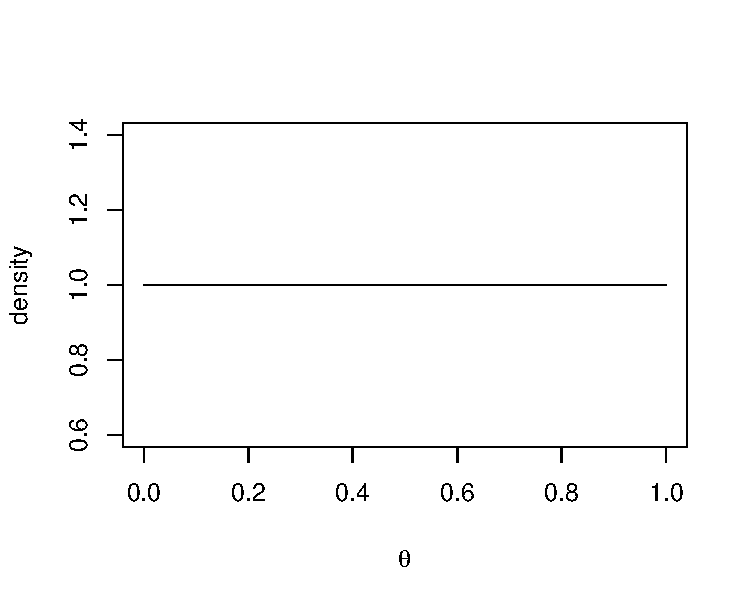
\includegraphics[width = .8\textwidth]{unif.pdf}
\caption{Unif(0,1) prior}
\label{fig:unif}
\end{figure}
}

\frame{

What happens if we consider though the transformation to $1/\theta.$ Is our prior still flat (does it place equal weight at every parameter value)?

}

\frame{

Suppose we consider Jeffreys' prior, $p_J(\theta),$ where $X \sim \text{Bin}(n,\theta).$ 

\vskip 1em

We calculate Jeffreys' prior by finding the Fisher information. The Fisher information tells us how much information the data gives us for certain parameter values. 

\vskip 1em
\begin{itemize}
\item Here, $p_J(\theta) \propto \text{Beta}(1/2,1/2).$ 
\item Let's consider the plot of this prior. Flat here is a purely abstract idea. 
\item In order to achieve objective inference, we need to compensate more for values on the boundary than values in the middle.
\end{itemize}
}

\frame{
\begin{figure}[htdp]
\centering
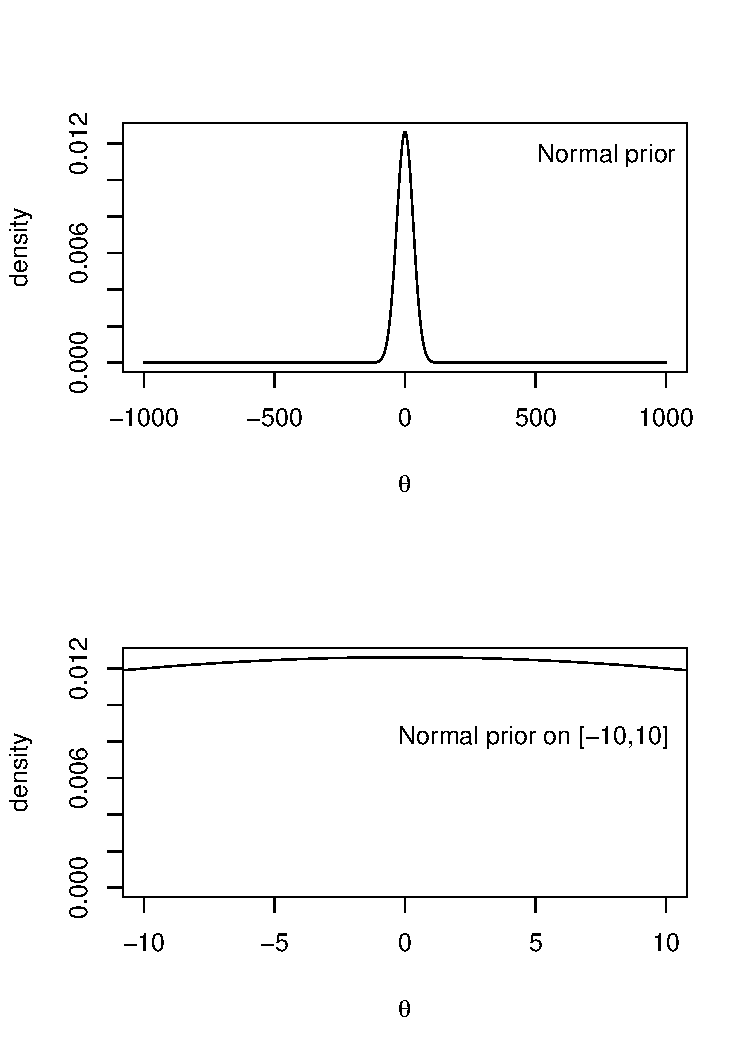
\includegraphics[width = .5\textwidth]{norm.pdf}
\caption{Normal priors}
\label{fig:unif}
\end{figure}
}

%\frame{
%\frametitle{My translation of Bayes}
%
%(Thomas Bayes)
%\begin{itemize}
%\item In 1763, Thomas Bayes considered the question of what prior to use when estimating a binomial success probability $p.$ 
%\item He described the problem quite differently back then by considering throwing balls onto a billiard table. He separated the billiard table into many different intervals and considered different events. 
%\item By doing so (and not going into the details of this), he argued that a Uniform(0,1) prior was appropriate for~$p.$
%\end{itemize}
%
%}

\frame{
\frametitle{The Frenchmen, Laplace}
(Laplace) In 1814, Pierre-Simon Laplace wanted to know the probability that the sun will rise tomorrow. He answered this question using the following Bayesian analysis:
\begin{itemize}
\item Let $X$ represent the number of days the sun rises. Let $p$ be the probability the sun will rise tomorrow. 
\item Let $X|p \sim \text{Bin}(n,p).$
\item Suppose $p \sim \text{Uniform}(0,1).$
\item Based on reading the Bible, Laplace computed the total number of days~$n$ in recorded history, and the number of days~$x$ on which the sun rose. Clearly, $x=n.$
\end{itemize}
}

\frame{
Then
\begin{align*}
\pi(p|x) &\propto \binom{n}{x}p^x(1-p)^{n-x}\cdot1\\
&\propto p^{x+1-1}(1-p)^{n-x+1-1}
\end{align*}
This implies $$p|x \sim \text{Beta}(x+1,n-x+1)$$
Then $$\hat{p} = E[p|x] = \frac{x+1}{x+1+n-x+1} = \frac{x+1}{n+2} = \frac{n+1}{n+2}.$$

}

\frame{
\begin{itemize}
\item Thus, Laplace's estimate for the probability that the sun rises tomorrow is $(n+1)/(n+2),$ where $n$ is the total number of days recorded in history. 
\item For instance, if so far we have encountered 100 days in the history of our universe, this would say that the probability the sun will rise tomorrow is $101/102 \approx 0.9902.$ 
\item However, we know that this calculation is ridiculous.  
\item Here, we have extremely strong subjective information (the laws of physics) that says it is extremely likely that the sun will rise tomorrow.  
\item Thus, objective Bayesian methods shouldn't be recklessly applied to every problem we study---especially when subjective information this strong is available.
\item \textcolor{blue}{If you have a philosophical question or debate, please come see me in office hours!}
\end{itemize}
}

\frame{
\frametitle{Criticism of the Uniform Prior}

\begin{itemize}
\item The Uniform prior of Bayes and Laplace and has been criticized for many different reasons. 
\item We will discuss one important reason for criticism and not go into the other reasons since they go beyond the scope of this course.

\item In statistics, it is often a good property when a rule for choosing a prior is \emph{invariant} under what are called one-to-one transformations. Invariant basically means unchanging in some sense.
%The invariance principle means that if I make some one-to-one transformation of a parameter, then the rule for choosing a prior for the original parameter corresponds to the rule for choosing a prior on the transformed version of the parameter.  For example, a rule that says ``put a Uniform prior on the parameter $p$'' is not invariant: if I instead consider $\log p,$ a Uniform prior for $\log p$ does not represent the same distribution as a Uniform prior of $p.$
\item The invariance principle means that a rule for choosing a prior should provide equivalent beliefs even if we consider a transformed version of our parameter, like $p^2$ or $\log p$ instead of $p.$
\end{itemize}


}

\frame{
\frametitle{Jeffreys' Prior}

One prior that is invariant under one-to-one transformations is Jeffreys' prior. 
%(\emph{Bayesian Data Analysis}, Gelman, \emph{et al.}, p.\ 63). You are \emph{not} responsible for this invariance proof (calculus is involved).

\vskip 1em

What does the invariance principle mean? 

\vskip 1em

Suppose our prior parameter is $\theta,$ however we would like to transform to $\phi.$ 

\vskip 1em

Define $\phi = f(\theta),$ where $f$ is a one-to-one function.

\vskip 1em

Jeffreys' prior says that if $\theta$ has the distribution specified by Jeffreys' prior for $\theta,$ then $f(\theta)$ will have the distribution specified by Jeffreys' prior for $\phi.$ We will clarify by going over two examples to illustrate this idea.

}

\frame{
\frametitle{Example: Uniform}

Note, for example, that if $\theta$ has a Uniform prior, Then one can show $\phi =f(\theta)$ will not have a Uniform prior (unless $f$ is the identity function). 

%Aside from the invariance property of Jeffreys' prior, in the univariate case, Jeffreys' prior satisfies many optimality criteria that statisticians are interested in.

}

\frame{
\frametitle{Example: Jeffreys'}
Define 
$$I(\theta) = -E\left[
\frac{\partial^2 \log p(y|\theta)}{\partial \theta^2}
\right],$$ where $I(\theta)$ is called the Fisher information. Then \emph{Jeffreys' prior} is defined to be
$$p_J(\theta) = \sqrt{I(\theta)}.$$

For homework you will prove that the uniform prior in not invariant to transformation but that Jeffrey's is. 
}

\frame{
\frametitle{Example: Jeffreys'}

Suppose 
\begin{align*}
X|\theta \sim \text{Binomial}(n,\theta).
\end{align*}
Let's calculate the posterior using Jeffreys' prior. To do so we need to calculate $I(\theta).$
Ignoring terms that don't depend on $\theta,$ we find
%\begin{align*}
%\log {p(x|\theta)} &= x\log{(\theta)} + (n-x)\log{(1-\theta)} \implies\\
%\frac{\partial \log p(x|\theta)}{\partial \theta}  &= \frac{x}{\theta} - \frac{n-x}{1-\theta}\\
%\frac{\partial^2 \log p(x|\theta)}{\partial \theta^2}  &= -\frac{x}{\theta^2} - \frac{n-x}{(1-\theta)^2}\\
%\end{align*}
\vskip 10em
}

%\frame{
%\frametitle{Example: Jeffreys'}
%\vskip 10em
%Since, $E(X) = n\theta,$ then
%$$I(\theta) = -E\left[-\dfrac{x}{\theta^2} - \dfrac{n-x}{(1-\theta)^2}\right] = 
%\dfrac{n\theta}{\theta^2} +\dfrac{n-n\theta}{(1-\theta)^2}
%= \dfrac{n}{\theta}  \dfrac{n}{(1-\theta)}
%= \dfrac{n}{\theta(1-\theta)}.$$
%This implies that
%\begin{align*}
%p_J(\theta) &= \sqrt{\frac{n}{\theta(1-\theta)}}\\
%&\propto \text{Beta}(1/2,1/2).
%\end{align*}
%
%
%
%}

\frame{
\begin{figure}[htdp]
\begin{center}
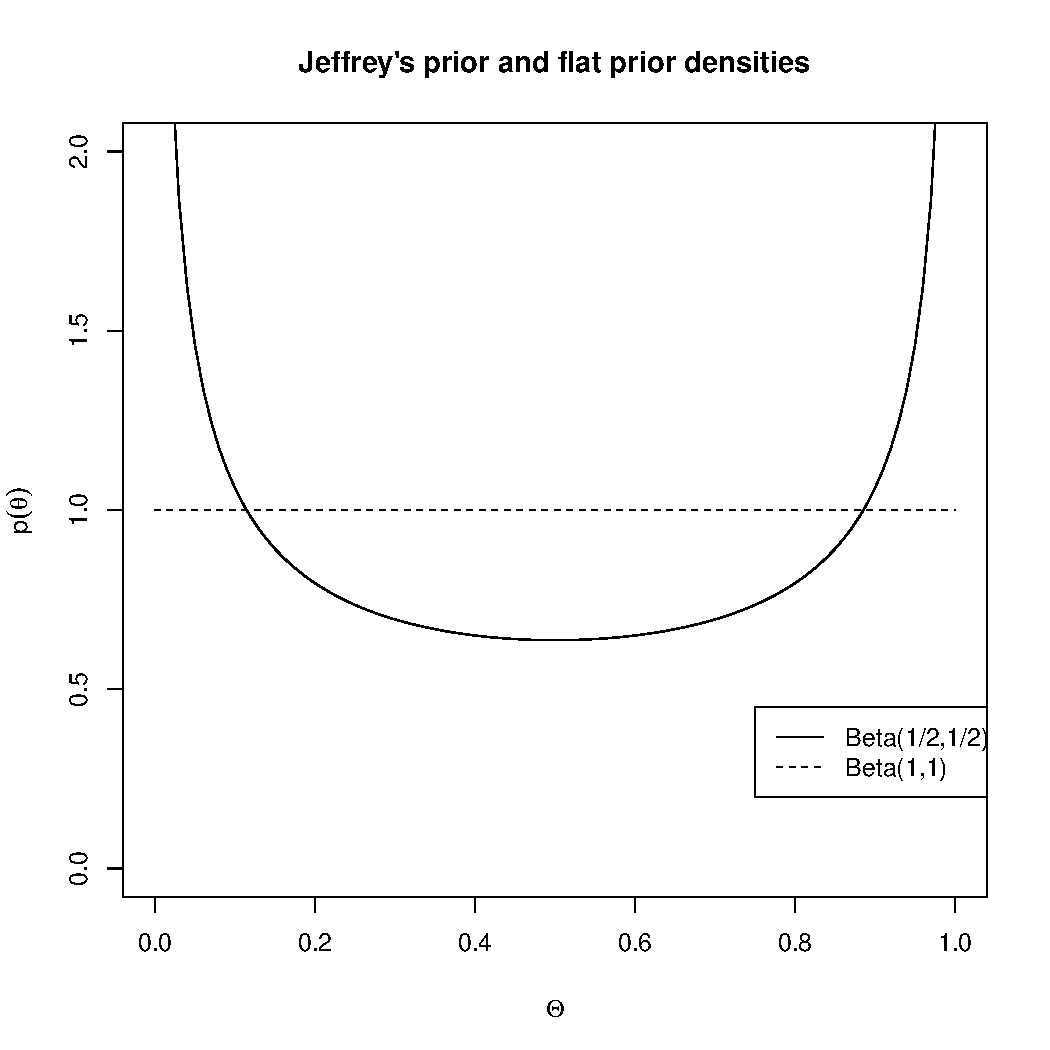
\includegraphics[width = .6\textwidth]{Lec7p2fig1.pdf}
\caption{Jeffreys' prior and flat prior densities}
\label{jeffreys}
\end{center}
\end{figure}
Figure~\ref{jeffreys} compares the prior density $\pi_J(\theta)$ with that for a flat prior, which is equivalent to a Beta(1,1) distribution. 
}

\frame{



%Note that in this case the prior is inversely proportional to the standard deviation. Why does this make sense?

\begin{itemize}
\item We see that the data has the least effect on the posterior when the true $\theta = 1,$ and has the greatest effect near 
the extremes, $\theta = 0$ or $1.$ 
\item Jeffreys' prior compensates for this by placing more mass near the extremes
of the range, where the data has the strongest effect. 
\item We could get the same effect by (for example) letting the prior be
$\pi(\theta) \propto \dfrac{1}{\text{Var}{\theta}}$ instead of $\pi(\theta) \propto \dfrac{1}{[\text{Var}{\theta}]^{1/2}}$. 
\item However, the former prior is not invariant under reparameterization, as we would prefer.
\end{itemize}
}

\frame{


We then find that
\begin{align*}
p(\theta \mid x) &\propto
\theta^x(1-\theta)^{n-x}\theta^{1/2-1}(1-\theta)^{1/2-1}\\
&=\theta^{x-1/2}(1-\theta)^{n-x-1/2}\\
&=\theta^{x-1/2+1-1}(1-\theta)^{n-x-1/2+1-1}.
\end{align*}
Thus, $\theta|x \sim \text{Beta}(x+1/2,n-x+1/2),$
which is a proper posterior since the prior is proper.\\ 
}

\frame{
\frametitle{Jeffreys' and Conjugacy}

\begin{itemize}
\item  In general, they are not conjugate priors.
\item For example, with a Gaussian model 
$X \sim N(\mu, \sigma^2),$ it can be shown that
$\pi_J(\mu) = 1$ and $\pi_J(\sigma) = \frac{1}{\sigma},$
which do not look anything like a Gaussian or an inverse gamma, respectively.
\item However, it can be shown that Jeffreys priors are limits of conjugate prior densities. 
\item For example, a Gaussian density $N(\mu_o,\sigma_o^2)$ approaches a flat prior as $\sigma_o^2 \rightarrow \infty$, while the inverse gamma 
$\sigma^{-(a+1)}e^{-b/\sigma}\to\sigma^{-1}$ as $a, b \rightarrow 0.$
\end{itemize}

}

\frame{
\frametitle{Limitations of Jeffreys'}

Jeffreys' priors work well for single-parameter models, but not for models with \textcolor{blue}{multidimensional parameters}. By analogy with the one-dimensional case, one might construct a naive Jeffreys prior as the joint density:
$$\pi_J(\theta) = |I(\theta)|^{1/2},$$
where $|\cdot|$ denotes the determinant and the $(i,j)$th element of the Fisher information matrix is given by
$$I(\theta)_{ij} = - E\left[
\frac{\partial^2 \log p(X|\theta)}{\partial \theta_i \partial \theta_j}
\right].$$
[For more reading: See PhD notes: Objective Bayes Chapter on reference priors, Gelman, et al. (2013)]
}

\frame{
Let's see what happens when we apply a Jeffreys' prior for $\theta$ to a multivariate Gaussian location model. Suppose 
$$X \sim N_p(\theta,I),$$ and we are interested in performing inference on $||\theta||^2.$ 
\begin{itemize}
\item In this case the Jeffreys' prior for 
$\theta$ is flat. 
\item It turns out that the posterior has the form of a non-central $\chi^2$ distribution with $p$ degrees of freedom. 
\item The posterior mean given one observation of $X$ is $E(||\theta||^2 \mid X) = ||X||^2 + p.$ \item This is not a good estimate because it adds $p$ to the square of the norm of $X,$ whereas we might normally want to shrink our estimate towards zero. 
\item By contrast, the minimum variance frequentist estimate of $ ||\theta||^2$ is $||X||^2 - p.$ 
\end{itemize}
[To learn more, Decision theory offered this fall, Read TPE, Lehmann and Casella, 2nd Ed.]

}

%\frame{
%\frametitle{Up next: Dealing with complex models}
%
%
%
%
%}


\end{document}